  Dieses Kapitel zeigt Methoden zur Analyse von Java Swing Applikationen.
  Dabei wird auf statische und dynamische Programmanalyse und das Problem bei
  der Verwendung von Bibliotheken eingegangen. Es existieren wahrscheinlich
  noch weitere Ansätze, welche hier nicht behandelt werden.
  
  \section{Grundlagen}
  
  Zur Analyse von bestehender Software gibt es verschiedene Ansätze. Aus dem
  Bereich der Qualitätssicherung kommt die Technik der statischen oder
  dynamischen Programmanalyse, siehe \cite{SoftwareanalyseBegriffeUndTechniken}
  S. 5. Die dynamische Programmanalyse wird darin unterteilt in White-Box-
  und Black-Box-Tests, siehe Abbildung \ref{img:programmanalyse}. In meiner
  Arbeit werde diese Methoden zur Analyse von Elementen der grafischen
  Benutzeroberfläche einsetzten.
  
  \begin{figure}[ht]
    \begin{center}
      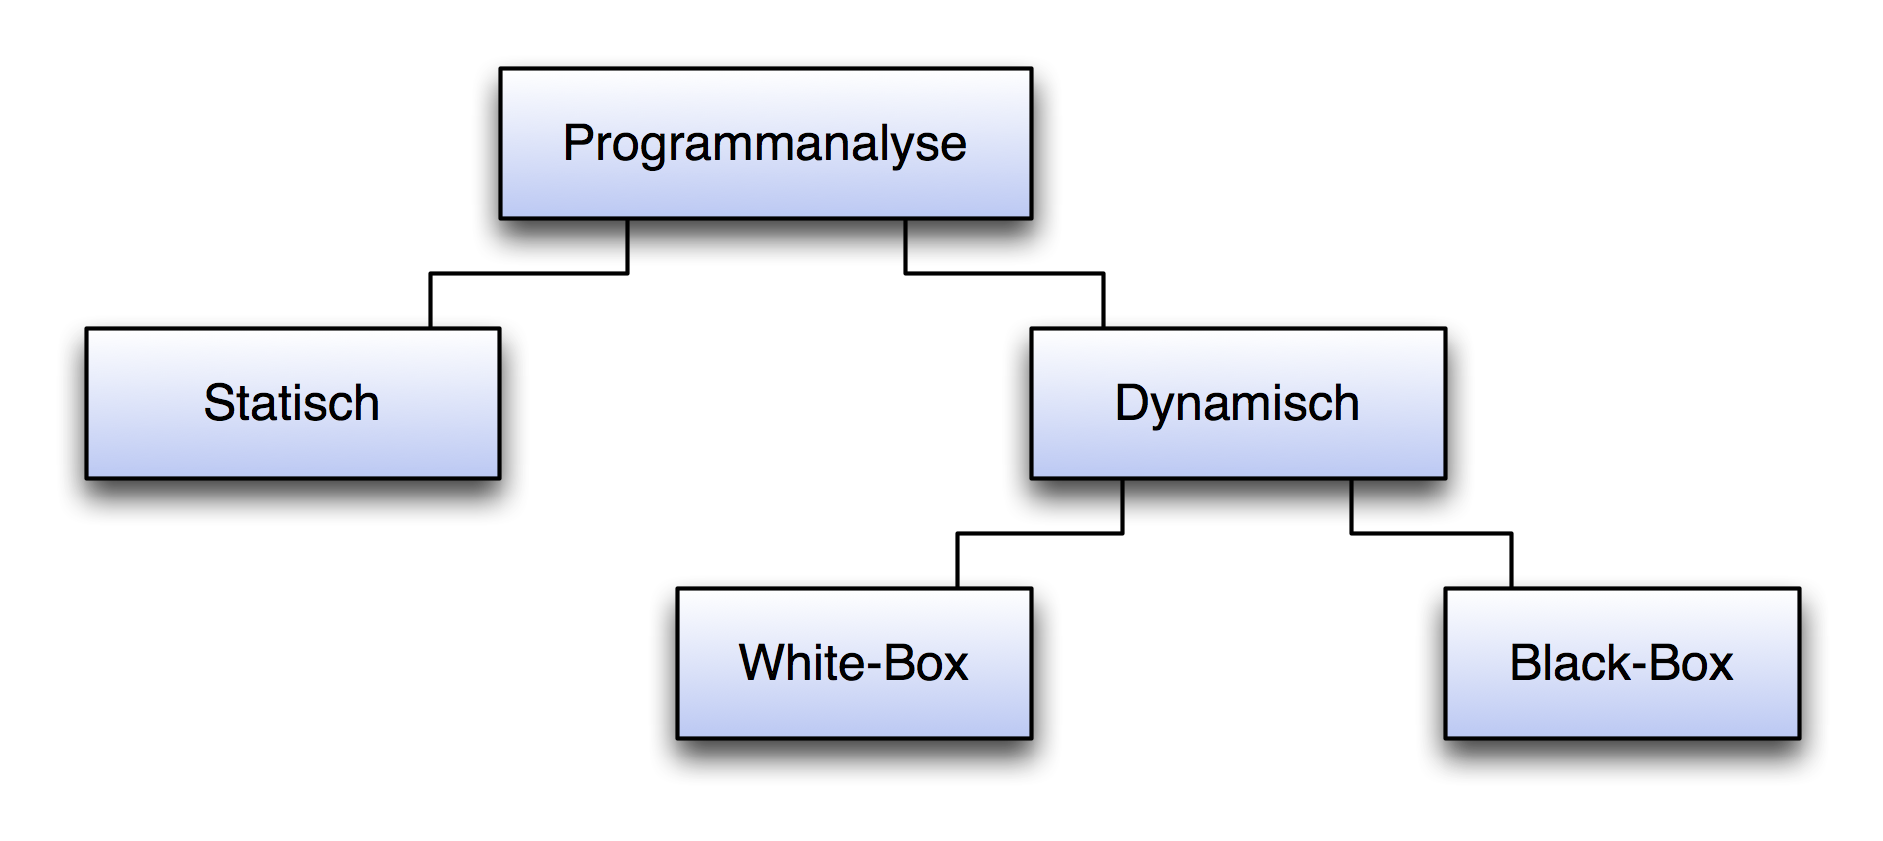
\includegraphics[width=0.6\textwidth]{./image/programmanalyse.png}
      \caption{Überblick über konventionelle Testmethoden (nach
      \cite{SoftwareanalyseBegriffeUndTechniken} S. 5)}
      \label{img:programmanalyse}
    \end{center}
  \end{figure}
  
  \subsection{Statische Programmanalyse}

  Die statische Programmanalyse basiert auf der Analyse des Sourcecodes. Das
  bedingt, dass der Sourcecode zugänglich ist. Als Softwareentwickler, kennt
  man das Verfahren eventuell aus der integrierten Entwicklungsumbegung
  (\acs{IDE})\acused{IDE}. Es gibt \acp{IDE}, wie zum Beispiel IntelliJ, siehe
  \cite{StaticCodeAnalysisIntelliJ}, die das Verfahren der statischen
  Programmanalyse nutzen. Wenn man Code schreibt, dann analysieren die
  \acp{IDE} den geschriebenen Code auf dessen syntaktische, semantische und
  lexikalische Informationen, siehe
  \cite{SoftwareQualitaetsmanagementInDerPraxis} S. 216f.
  
  Im Artikel \cite{GUIAnalysenUndBibliotheken} befasst sich der Author damit,
  was man bei \ac{GUI} lastiger Software durch eine statische Programmanaylse in
  Erfahrung bringen kann. Nach Aussage des Authors kann man bei deren
  Vorgeschlagenen Techniken folgendes erreichen:
  
  ``\begin{itshape}Im Rahmen dieser Analyse wird erkannt, welche Teile des
  Programms zur GUI gehören, welche Widgets das Programm enthält, welche
  Attribute, mit ihren Werten, diese Widgets besitzen, wie diese Widgets mit
  Events untereinander verbunden sind und wie sie in den einzelnen Fenstern der
  GUI strukturiert
  sind.\end{itshape}''\footnote{\cite{GUIAnalysenUndBibliotheken}
  Zusammenfassung - Seite 1}
    
  \subsection{Dynamische Programmanalyse}
  
  Bei der dynamischen Programmanalyse wird das zu analysierende Programm 
  ausgeführt. Die dynamische Programmanalyse wird in zwei Unterarten aufgeteilt,
  das Black-Box Verfahren und das White-Box Verfahren.
    
  \subsubsection{Black-Box Verfahren}
  
  Der Analyst hat keinerlei Informationen über das Innenleben des zu
  analysierenden Programms. Die Analyse basiert auf der intuitiven Bedienung der
  grafischen Oberfläche, durch den Analysten.
  
  \subsubsection{White-Box Verfahren}
  
  Der Analyst hat explizite Kenntnisse über das Innenleben des zu
  analysierenden Programms, zudem steht ihm der Sourcecode zur Verfügung. Mit
  der Hilfe des Sourcecodes können sinnvolle Schlüsse im Bezug auf die Analyse
  getroffen werden, da Spezialfälle, welche nicht offensichtlich sind,
  analysiert werden können. Als Beispiel dafür, möchte ich eine kurze
  Codesequenz zeigen, siehe Listing \ref{lst:dreifacherMausklick} Zeile 4.
  Dabei wird auf einen dreifachen Mausklick abgefragt. Da ein solches Verhalten nicht
  intuitiv ist, würde das ohne Sourcecode wahrscheinlich nicht gefunden werden.:
  \newline
  %\newpage
  
  \begin{lstlisting}[
    captionpos=b,
    caption=Spezialfall - dreifacher Mausklick,
    label=lst:dreifacherMausklick
  ]
  component.addMouseListener(new MouseAdapter() {
    public void mouseClicked(MouseEvent evt) {
      if (evt.getClickCount() == 3) {
        System.out.println("triple-click");
      }
    }
  });
  \end{lstlisting}
  
  \subsection{Probleme bei der Verwendung von Bibliotheken}
  
  Gemäss \cite{GUIAnalysenUndBibliotheken} S. 1f. besteht ebenfalls ein Problem
  bei der Verwendung von Bibliotheken. Die Grundproblematik besteht darin,
  dass eine Bibliothek eventuell ohne Zugriff auf deren Sourcecode verwendet
  wird. Damit wird das Verfahren der statischen Programmanalyse und der
  dynamischen White-Box Programmanalyse unmöglich.
  
  Falls eine statische Programmanalyse angestrebt wird, und der Sourcecode der
  verwendeten Bibliotheken vorhanden ist, kann sich das negativ auf die
  Präzision der Analyse auswirken. Denn es ist üblich, dass Bibliotheken
  meisst um ein Vielfaches grösser sind als das zu analysierende Programm. Der
  Aufwand wird durch die grössere Menge an Sourcecode zudem erhöht.
  
  \section{Wahl des Verfahrens}
  
  Die Wahl des Verfahrens der Analyse soll wie in der Abbildung
  \ref{img:guiAnalyse} durchgeführt werden. Leider wurde während der
  Durchführung der Diplomarbeit kein sinnvoll einsetzbares Werkzeug zur
  statischen Programmanalyse für Java Swing Applikationen gefunden. Somit wurde
  im Falle von vorhandenem Quellcode nur das dynamische White-Box Verfahren
  angewendet.
  
  \begin{figure}[ht]
    \begin{center}
      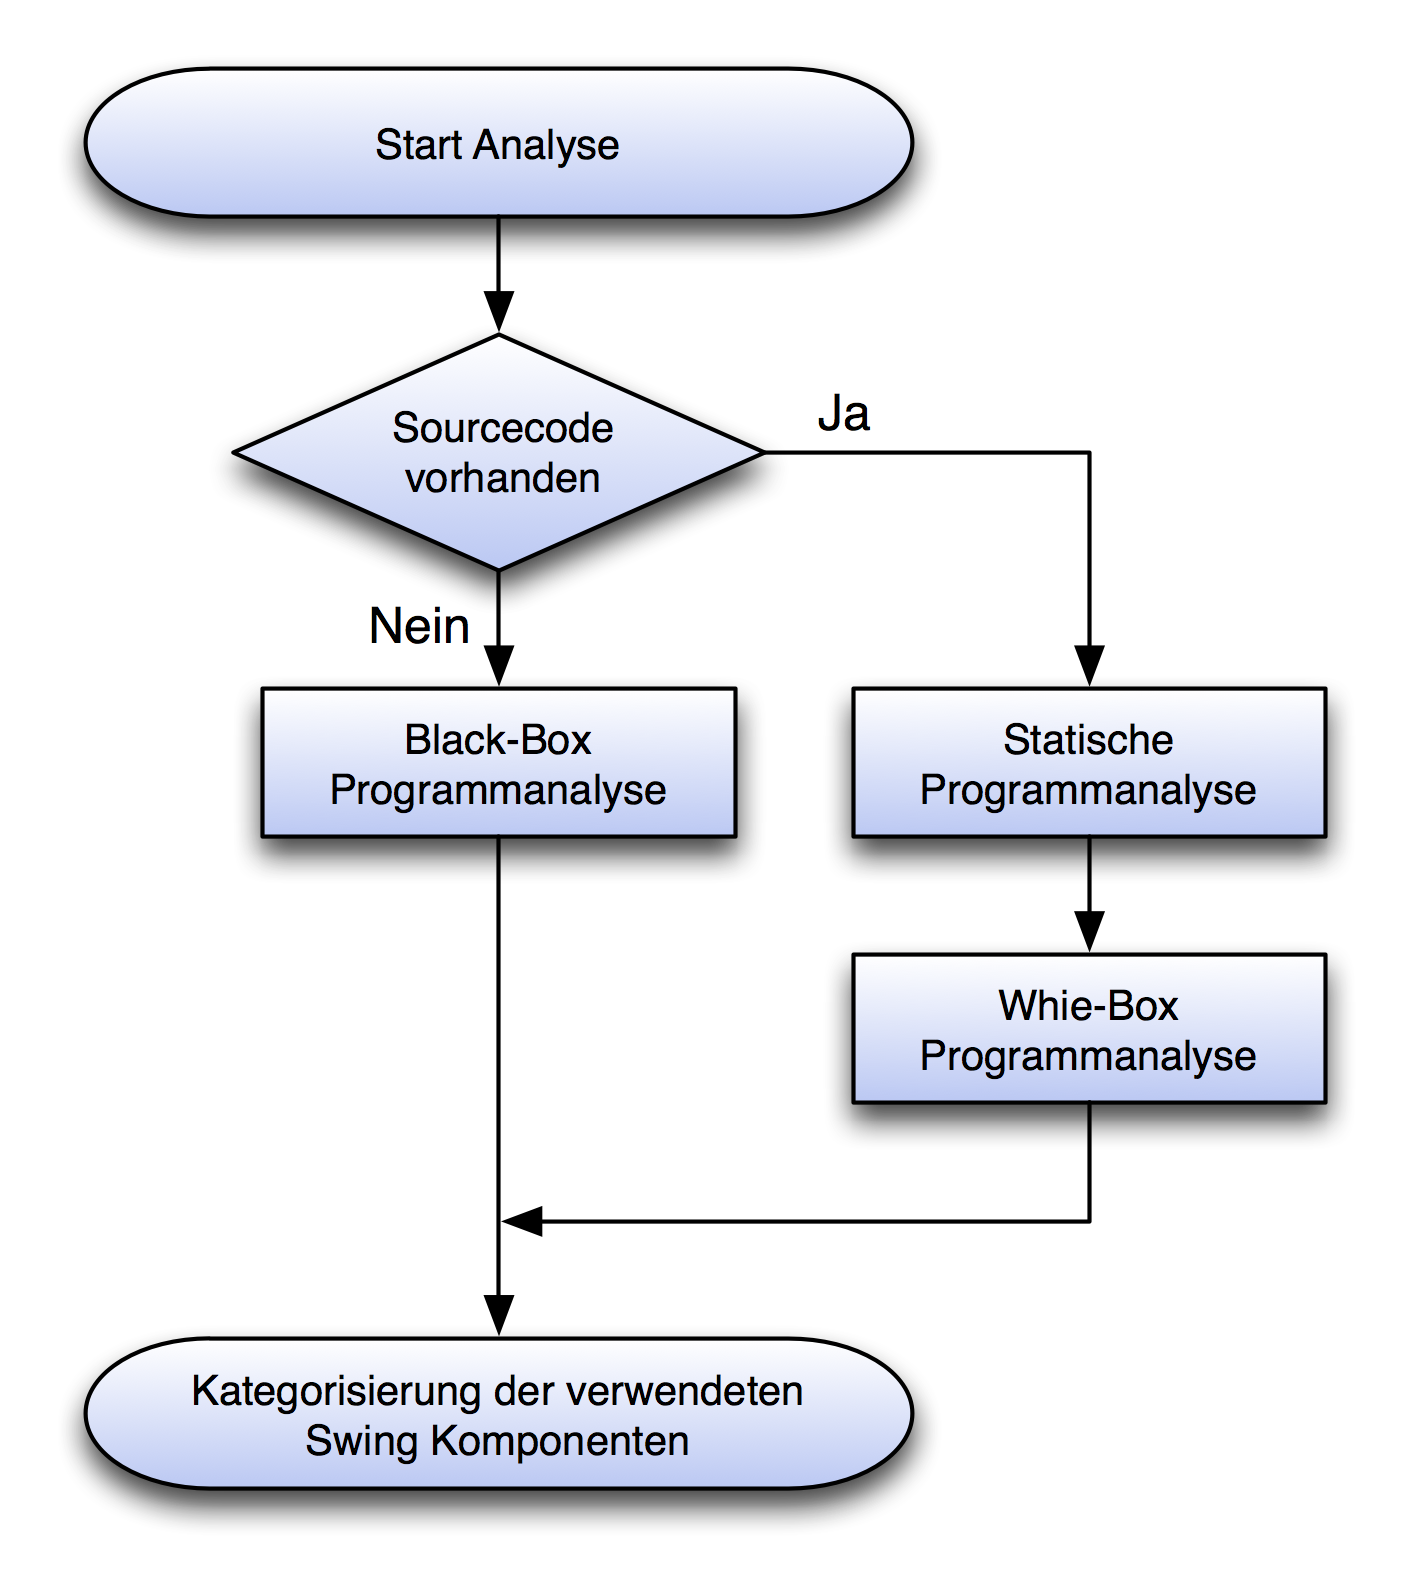
\includegraphics[width=0.5\textwidth]{./image/guiAnalyse.png}
      \caption{Wahl des Verfahrens der Programmanalyse}
      \label{img:guiAnalyse}
    \end{center}
  \end{figure}